\begin{question}[ID=Gunslinger,type=exam]{20}
  \textbf{Baysian Games:}
  Consider a Wild West shootout between Earp and the Stranger. \\
  With probability .75, the Stranger is a Gunslinger type and the table shows Earp's and the Stranger's payoffs
  \begin{table}[!h]
  \begin{center}
    \begin{tabular}{*{4}{c|}}
      \multicolumn{2}{c}{} &
      \multicolumn{2}{c}{Gunslinger Stranger} \\ \cline{3-4}
      \multicolumn{1}{c}{} &                & Draw & Wait \\ \cline{2-4}
      \multirow{2}*{Earp} & Draw & 2, 3 & 3, 1 \\ \cline{2-4}
                                     & Wait & 1, 4 & 8, 2 \\ \cline{2-4} 
    \end{tabular}
  \end{center}
  \end{table} \\
  But with probability .25, the Stranger is a Cowpoke type and the table shows Earp's and the Stranger's payoffs
  \begin{table}[!h]
  \begin{center}
    \begin{tabular}{*{4}{c|}}
      \multicolumn{2}{c}{} &
      \multicolumn{2}{c}{Cowpoke Stranger} \\ \cline{3-4}
      \multicolumn{1}{c}{} &             & Draw & Wait \\ \cline{2-4}
      \multirow{2}*{Earp} & Draw & 5, 2 & 4, 1 \\ \cline{2-4}
                                  & Wait & 6, 3 & 8, 4 \\ \cline{2-4} 
    \end{tabular}
  \end{center}
  \end{table}
  \begin{tasks}
    \task (\points{4}) 
    What is the Nash equilibrium \textbf{when the Stranger is always a Gunslinger}? \\
    \PrintSolutionsTF{
    \fbox{ \parbox{\linewidth}{
        \textbf{NE:} \{Earp \texttt{Draw}s, Gunslinger \texttt{Draw}s\}
      } } }{\vspace{2cm}} 
    \task (\points{4})
    What is the Nash equilibrium \textbf{when the Stranger is always a Cowpoke}? \\
    \PrintSolutionsTF{
    \fbox{ \parbox{\linewidth}{
        \textbf{NE:} \{Earp \texttt{Wait}s, Gunslinger \texttt{Wait}s\}
      } } }{\vspace{2cm}}
    \task (\points{4}) 
    What is the Nash equilibrium when Earp believes the Stranger is a 
    \textbf{Gunslinger with probability 0.75}? \\
    \PrintSolutionsTF{
    \fbox{ \parbox{\linewidth}{
        \begin{align*}
          EU_{\text{Earp}}(\text{Draw}) & = 3/4 (2) + 1/4 (4) = 2.5 \\
          EU_{\text{Earp}}(\text{Wait}) & = 3/4 (1) + 1/4 (8) = 2.75 \\
        \end{align*}
        So Earp should wait if he believes it is likely enough he is against a Gunslinger. \\
        \textbf{BNE:} \{(Earp \texttt{Waits}, believing that prob Stranger is Gunslinger is .75),
        (Cowpoke \texttt{Waits}, Gunslinger \texttt{Draws}) \}
      } } }{\vspace{3cm}}
    \task (\points{4})
    Consider a strategic move variation where the Gunslinger can commit to only playing Wait 
    before Nature has assigned them a type. \\
    Is this type of commitment \textit{credible}? Why or why not?\\
    \PrintSolutionsTF{
    \fbox{ \parbox{\linewidth}{
        Not credible for the Gunslinger to commit to \texttt{Wait}
        because \texttt{Draw} strictly dominates \texttt{Wait}.
      } } }{\vspace{3cm}}
  \end{tasks}
\end{question}

\newpage

\begin{question}[ID=StudentBoard,type=exam]{12}
\textbf{Bayesian Game:}
Consider a situation in which a student can decide to cheat or be honest on an exam.
If the faculty thinks the student has cheated, 
the faculty member has to decide whether to expel them from the college
or refer them to the Honor Board. 
The Honor Board has to decide whether to expel the student or find them innocent.
The payoffs are ordered, student, faculty, and college.
Assume the board shares the college's payoffs. 
% \footnote{Cliff Bekar, Lewis and Clark College}
\begin{figure}[!h]
  \centering
  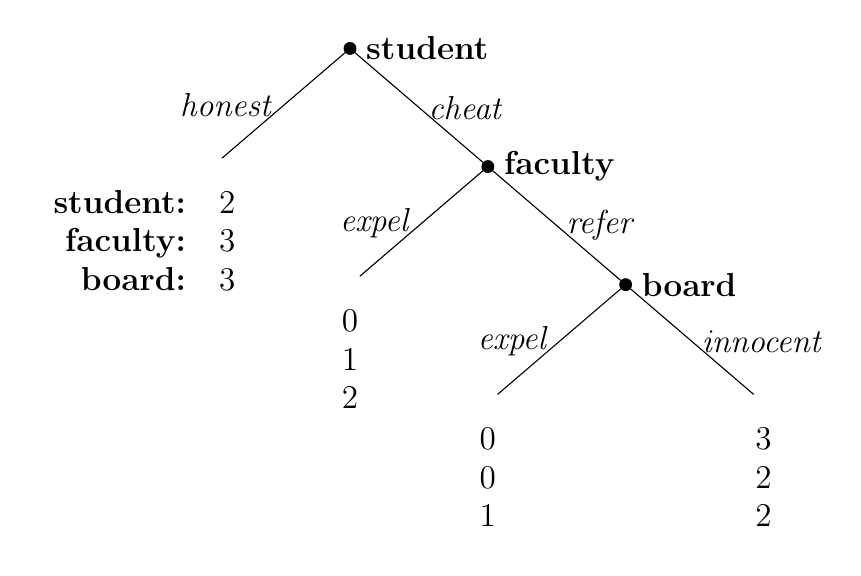
\begin{tikzpicture}[scale=1.0,font=\large]
  \tikzstyle{solid node}=[circle,draw,inner sep=1.5,fill=black]
  \tikzstyle{level 1}=[level distance=15mm,sibling distance=3.5cm]
  \tikzstyle{level 2}=[level distance=15mm,sibling distance=3.5cm]
  \tikzstyle{level 3}=[level distance=15mm,sibling distance=3.5cm]
  \node(0)[solid node,label=right:{\textbf{student}}]{}
      child{node[label=below:{
              \begin{tabular}{rlc}
                \textbf{student:} & {2}&  \\
                \textbf{faculty:} & {3}&  \\
                \textbf{board:} & {3}& \hspace{1.3cm} \\
              \end{tabular}
          }]{} 
      edge from parent node[left]{\textit{honest}}}
      child{node[solid node,label=right:{\textbf{faculty}}]{} 
          child{node(1)[label=below:{
              \begin{tabular}{c}
                   {0}  \\
                   {1} \\
                   {2} \\
              \end{tabular}
          }]{} 
          edge from parent node[left]{\textit{expel}} 
          }
          child{node(2)[solid node, label=right:{\textbf{board}}]{} 
              child{node[label=below:{
                  \begin{tabular}{c}
                      {0} \\
                      {0} \\
                      {1} \\
                  \end{tabular}
                  }]{} 
              edge from parent node[left]{\textit{expel}} 
              }
              child{node[label=below:{
                  \begin{tabular}{c}
                       {3} \\
                       {2} \\
                       {2} \\
                  \end{tabular}
              }]{} 
              edge from parent node[right]{\textit{innocent}} 
              }
          edge from parent node[right]{\textit{refer}} 
          }
      edge from parent node[right]{\textit{cheat}}
      };
  \end{tikzpicture}
\end{figure}
\begin{tasks}
  \task (\points{4}) 
  Find the Subgame Perfect Nash Equilibrium. \\
  \PrintSolutionsTF{
  \fbox{
    \parbox{\linewidth}{
      Backwards Induction:
      \begin{itemize}
        \item \textbf{board} will find $innocent$
        \item \textbf{faculty} will $refer$ knowing board will find $innocent$
        \item \textbf{student} will $cheat$ knowing faculty will refer, board will find innocent.
      \end{itemize}
      \textbf{SPNE:} \{$cheat$, $refer$, $innocent$\}
    }
  }
  }{\vspace{4cm}}
  \task (\points{4}) 
  Assume now that the board acts like $Nature$, making no deliberate choice 
  but instead expels a guilty student $q\%$ of the time.
  Solve for the range of $q$ such that the student chooses $honest$ in the SPNE. \\
  \PrintSolutionsTF{ \fbox{\parbox{\linewidth}{
    If board acts randomly, \textbf{faculty} will $expel$ when:
    \begin{align*}
      EU_f(expel) & \geq EU_f(refer) \\
      1 & \geq 0q + 2(1-q) \\
      1 & \geq 2 - 2q \\
      q & \geq 1/2
    \end{align*}
  }}}{\vspace{4cm}}
  \task (\points{4}) 
  Relative to the pure threat of explusion alone, who gains and who loses
  from the existence of an honor board that expels probabalistically? \\
  \PrintSolutionsTF{ \fbox{\parbox{\linewidth}{
    Student loses, because they get their 2nd favorite outcome instead of favorite.
    Faculty and board both gain because their favorite outcome is achieved in equilibrium.
  }}}{}
\end{tasks}
\end{question}
\newpage

%------------------------------------------------------------------

\begin{question}[ID=Signaling,type=exam]{16}
  \textbf{Signaling:}
  Consider a Bayesian game where Nature determines whether an employee
  is an A type and more suited for executive roles
  or a B type who are more suited for janitorial work.
  The Manager cannot observe the hidden type of an employee,
  but employees may choose to go to college or not. \\
  The extensive form game is shown below: \\
  \begin{center}
  \begin{tikzpicture}[edge from parent/.style={draw, very thick}]
    \tikzstyle{solid node}=[circle,draw,inner sep=1.5,fill=black]
    \tikzstyle{hollow node}=[circle,draw,inner sep=.25]
    \tikzstyle{level 1}=[level distance=10mm,sibling distance=8cm]
    \tikzstyle{level 2}=[level distance=20mm,sibling distance=3cm]
    \tikzstyle{level 3}=[level distance=20mm,sibling distance=2cm]
    \tikzstyle{pruned edge from parent}=[draw, very thick, blue, dashed, -]
    \node(0)[solid node,label=above:{Nature}]{}
        child{node(1)[solid node,label=left:{Employee}]{}
            child{node(3)[hollow node,label=below:{
                \begin{tabular}{rlc}
                     Employee: & 0 & \hspace{1.2cm} \\
                     Manager:  & 5 &
                \end{tabular}
            }]{} edge from parent node[left]{\texttt{Trade School}}}
            child{node(4)[solid node]{}
                child{node[hollow node,label=below:{
                    \begin{tabular}{c}
                         10  \\
                         10
                    \end{tabular}
                }]{} edge from parent node[left]{\texttt{Executive}}}
                child{node[hollow node,label=below:{
                    \begin{tabular}{c}
                         5  \\
                         5
                    \end{tabular}
                }]{} edge from parent node[right]{\texttt{Janitor}}}
            edge from parent node[right]{\texttt{College}}}
            edge from parent node[left,xshift=0,yshift=5]{Type A (p)}
        }
        child{node(2)[solid node,label=right:{Employee}]{}
            child{node(6)[solid node,label=right:{}]{}
                child{node[hollow node,label=below:{
                    \begin{tabular}{c}
                         10  \\
                         0 
                    \end{tabular}
                }]{} edge from parent node[left]{\texttt{Executive}}}
                child{node[hollow node,label=below:{
                    \begin{tabular}{c}
                         5  \\
                         10
                    \end{tabular}
                }]{} edge from parent node[right]{\texttt{Janitor}}}
            edge from parent node[left]{\texttt{College}}}
            child{node(5)[hollow node,label=below:{
              \begin{tabular}{c}
                8  \\
                5
              \end{tabular}
            }]{}
            edge from parent node[right]{\texttt{Trade School}}}
            edge from parent node[right,xshift=0,yshift=5]{Type B (1-p)}
        }
        ;
  % information set
  \draw[dashed,rounded corners=7]($(4)+(-.2,.25)$)rectangle($(6)+(.2,-.25)$);
  % specify movers
  \node at ($.5*(4)+.5*(6)$) {Manager};
  \end{tikzpicture}
\end{center}
  \begin{tasks}
    \task (\points{4})
    Suppose that $p=3/4$.
    Suppose that the Manager's pure strategy is to always hire College grads as 
    \textit{Executive}s.
    Solve for the Subgame-perfect Bayes-Nash Equilibrium (SPBNE). \\
    Is this a \textit{separating} or a \textit{pooling} equilibrium? \\
    \PrintSolutionsTF{ \fbox{\parbox{\linewidth}{
      \underline{Case 1: If Managers always hire College grads as \textit{Executives}:}
      \begin{align*}
        EU_{\text{A}}(\texttt{College}) & = \underline{10} \\
        EU_{\text{A}}(\texttt{Trade School}) & = 0 \\
        EU_{\text{B}}(\texttt{College}) & = \underline{10} \\
        EU_{\text{B}}(\texttt{Trade School}) & = 8 \\
      \end{align*}
      So Manager should believe that all employees will go to college,
      $prob(\text{College}|\text{A}) = 
      prob(\text{College}|\text{B}) = 1$. \\
      \begin{align*}
        EU_{\text{Manager}}(\texttt{Executive}|\text{College}) & 
        = 10\left(\frac{1\times p}{p + (1-p)}\right) + 0 \left(\frac{1\times (1-p)}{p + (1-p)}\right) 
        = 10p  = 10(3/4) = \underline{7.5} \\
        EU_{\text{Manager}}(\texttt{Janitor}|\text{College}) & 
        = 5\left(\frac{1\times p}{p + (1-p)}\right) + 10 \left(\frac{1\times (1-p)}{p + (1-p)}\right)
        = 10-5(3/4) = 6.25 \\
      \end{align*}
      \textbf{\textit{Pooling} SPBNE:} 
      \begin{itemize}
        \item Manager: hire \texttt{Executive} 
        with the belief that prob(A$|$College) = $3/4$.
        \item Employee: \texttt{College} if Type A, \texttt{College} if Type B 
        with the belief that prob(Executive$|$College) = 1.
      \end{itemize}
    }}}{\vspace{4cm}}
    \task (\points{4})
    Suppose that $p=3/4$.
    Is there a \textit{separating equilibrium} in pure strategies
    where all A types go to college,
    and all B types go to trade schools? \\
    \PrintSolutionsTF{ \fbox{\parbox{\linewidth}{
      If Manager believes that all Type As go to college,
      $prob(\text{College}|\text{A}) = 1$,
      and all Type Bs go to trade schools;
      $prob(\text{College}|\text{B}) = 0$,
      then they should only hire \texttt{Executive}s. \\
      \begin{align*}
        EU_{\text{Manager}}(\texttt{Executive}|\text{College}) & 
        = 10\left(\frac{1\times p}{p + 0}\right) + 0 \left(\frac{1\times 0}{p + 0}\right) 
        = \underline{10} \\
        EU_{\text{Manager}}(\texttt{Janitor}|\text{College}) & 
        = 5\left(\frac{1\times p}{p + 0}\right) + 5 \left(\frac{1\times 0}{p + 0}\right)
        = 5 \\
      \end{align*}
      However, if Employees believe that the chances of being hired as executives
      conditional on choosing \texttt{College} is equal to 1,
      then they will all pool in the \texttt{College} strategy
      as in part (a). \\
      \textbf{No separating equilibrium in pure strategies}
    }}}{\vspace{4cm}}
    \task (\points{4})
    Suppose that now $p=2/3$ so that Managers are indifferent 
    between hiring a random employee as a \texttt{Executive} or as a \texttt{Janitor}. \\
    Define mixed strategies for both players and use them to solve for a
    \textit{semi-separating} equilibrium. \\
    \PrintSolutionsTF{ \fbox{\parbox{\linewidth}{
      Let $q$ be the probability a Manager hires on an \texttt{Executive}.
      \begin{align*}
        EU_{\text{A}}(\texttt{College}) & = \underline{10q + 5(1-q)} \\
        EU_{\text{A}}(\texttt{Trade School}) & = 0 \\
        EU_{\text{B}}(\texttt{College}) & = \underline{10q + 5(1-q)} \\
        EU_{\text{B}}(\texttt{Trade School}) & = \underline{8} \\
      \end{align*}
      Type As will always go to college,
      but Type Bs will only go to college if $10q + 5(1-q) > 8$,
      and will mix if their expected utilities 
      from college and trade school are equal.
      \begin{align*}
        10q + 5(1-q) & = 8 \\
        % 5q & = 3 \\
        \Rightarrow q  & = 3/5
      \end{align*}
      Now let $r$ be the probability that a Type B Employee goes to College.
      \begin{align*}
        EU_{\text{Manager}}(\texttt{Executive}|\text{College}) & 
        = 10\left(\frac{1\times 2/3}{2/3 + 1/3(r)}\right) + 0 \left(\frac{r\times 1/3}{2/3 + 1/3(r)}\right) 
        = 10 \frac{2}{2+r} \\
        EU_{\text{Manager}}(\texttt{Janitor}|\text{College}) & 
        = 5\left(\frac{1\times 2/3}{2/3 + 1/3(r)}\right) + 10 \left(\frac{r\times 1/3}{2/3 + 1/3(r)}\right) 
        = 5 \frac{2}{2+r} + 10 \frac{r}{2+r} \\
      \end{align*}
      So a Manager will be willing to mix their hiring 
      between executives and janitors when:
      $$20 = 10 + 10r \Rightarrow r = 1/2$$
      \textbf{\textit{Semi-separating} SPBNE:}
      \begin{itemize}
        \item Manager's mixed strategy: hire \texttt{Executive} with probability 3/5, \texttt{Janitor} with 2/5 probability,
        \begin{itemize}
          \item beliefs: prob(A$|$College) 
          = $\frac{(1)(2/3)}{(1)(2/3)+(1/2)(1/3)} = \frac{2}{5/2} = 4/5$
        \end{itemize}
        \item Employee's strategy: 
        \begin{itemize}
          \item if Type A $\rightarrow$ \texttt{College}, 
          \item if Type B $\rightarrow$
        (\texttt{College} with prob 1/2, \texttt{Trade School} with prob 1/2)
        \item beliefs: probability of being hired as \texttt{Executive} after college = 3/5
        \end{itemize}
      \end{itemize}
    }}}{\vspace{12cm}}
    \task (\points{4})
    What is the \textit{signalling} value of an employee choosing \texttt{College}?
    Use Bayes rule to compare the ex-ante probability $p=2/3$ of a Type A
    to the updated belief of a Manager as to the Employee being Type A 
    conditional on observing college
    in the semi-separating equilibrium in part (c).
    \PrintSolutionsTF{ \fbox{\parbox{\linewidth}{
      In the semi-separating equilibrium above, the \texttt{College} strategy has signaling value. \\
      The signal of college gives the Manager a better idea of the Employee's true type than their naive estimate of $p=2/3$.
      $$
      prob(\text{A} | \texttt{College}) = 
        \frac{prob(\texttt{College}|\text{A})\times prob(\text{A})}{prob(\texttt{College})} =
        \frac{1\times p}{1p + r(1-p)} =
        4/5 > p = 2/3
    $$
    This is because all Type A's choose college in equilibrium,
    but only a fraction, $r=1/2$, of Type B's choose college.
    }}}{}
  \end{tasks}
\end{question}